\documentclass{article}
\author{Wenzhao Xu (Environmental Engineering)\\ Haoyan Cai (Statistics) }
\title{STAT 542 Final Project Proposal}
\usepackage{amsmath}
\usepackage{graphicx}
\usepackage{subfig}
\usepackage{multirow}
\usepackage[top=1in, bottom=1in, left=1.25in, right=1.25in]{geometry}

\begin{document}
	\maketitle
	
	\section{Introduction} % (fold)
	\label{sec:introduction}
	
	\paragraph{} The data are about accelerometer data from mobile devices. The train data contain X,Y,Z axis acceleration values from 387 devices and testing data set consists of 90024 testing sequences. Each test sequence comes with a proposed device Id. The goal is to judge whether the claimed device is the true device that produces the test sequence. 
	% section introduction (end)
	
	\section{Data Set} % (fold)
	\label{sec:section_name}
	\paragraph{}
	Package "ff" and SQL database can be used to import data from a large csv file. Unix time is then converted to standard GMT time. A typical visulization of data is shown in Figure 1, in which Device 7 is a device with long sampling time and total 523187 points while Device 770 has limited sampling points of 28475. 
	\begin{figure}
		\centering
		\subfloat[Device 770]{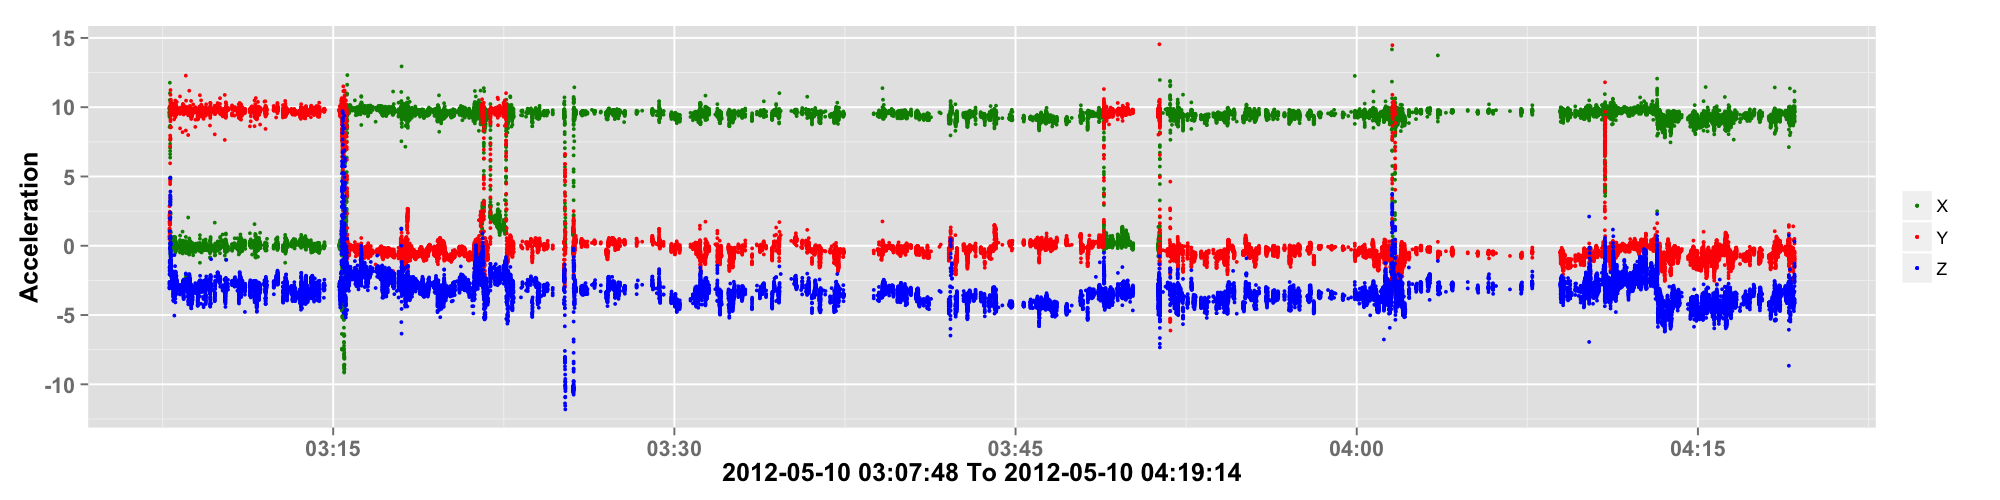
\includegraphics[width=1\textwidth]{photoshare/770.png}}\\
		\subfloat[Device 7]{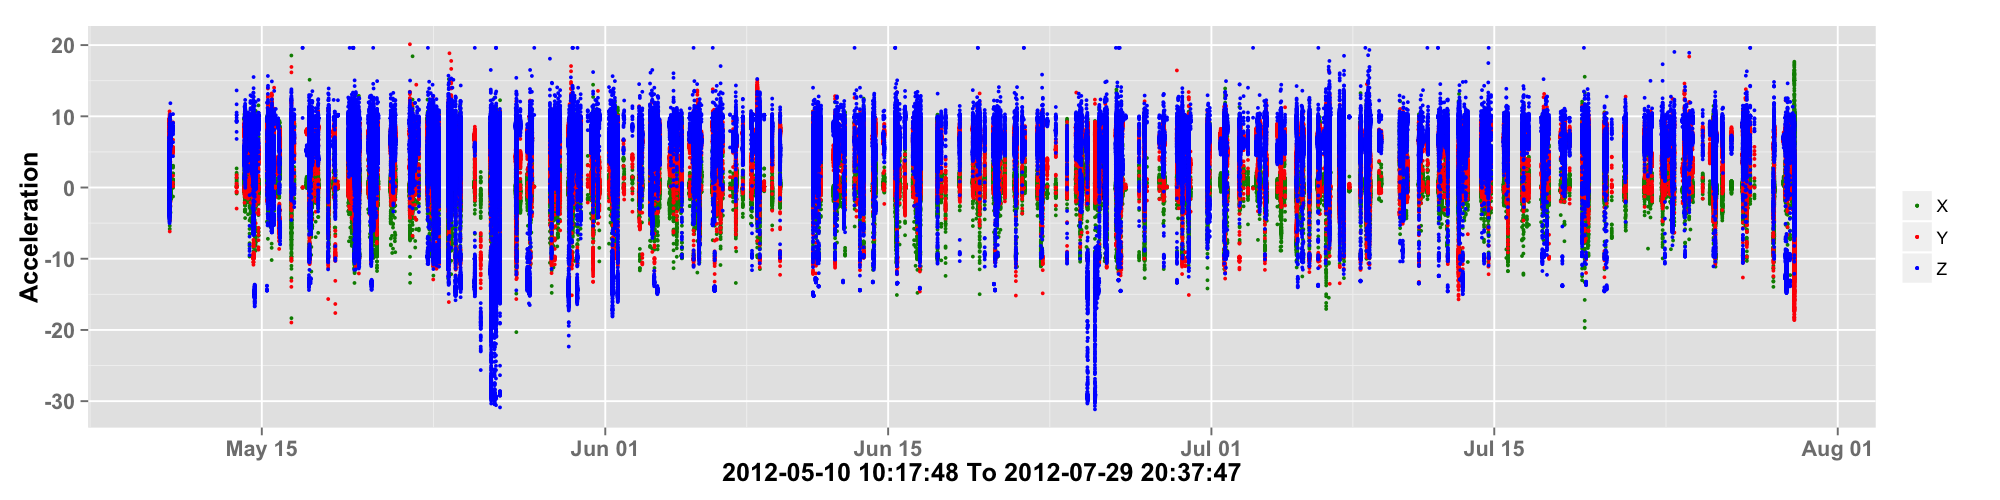
\includegraphics[width=1\textwidth]{photoshare/7.png}} \\
		\caption{Acceleration Data Along Time}
	\end{figure}
	
	\paragraph{}In test data, each sequence contains 300 sampling points, roughly lasts for less than 1 minute. We need to identify whether the professed device in the test sequence is the true device. Figure 2 shows two sequence whose professed device are 770. Compared with the train data from device 770 (Fig 1(a)), it seems sequence 838966 is likely belong to device 770 while sequence 690194 is not since the range of X,Y,Z in sequence 838966 is consistent with training data from device 770. 
	\begin{figure}
		\centering
		\subfloat[Sequence 690194]{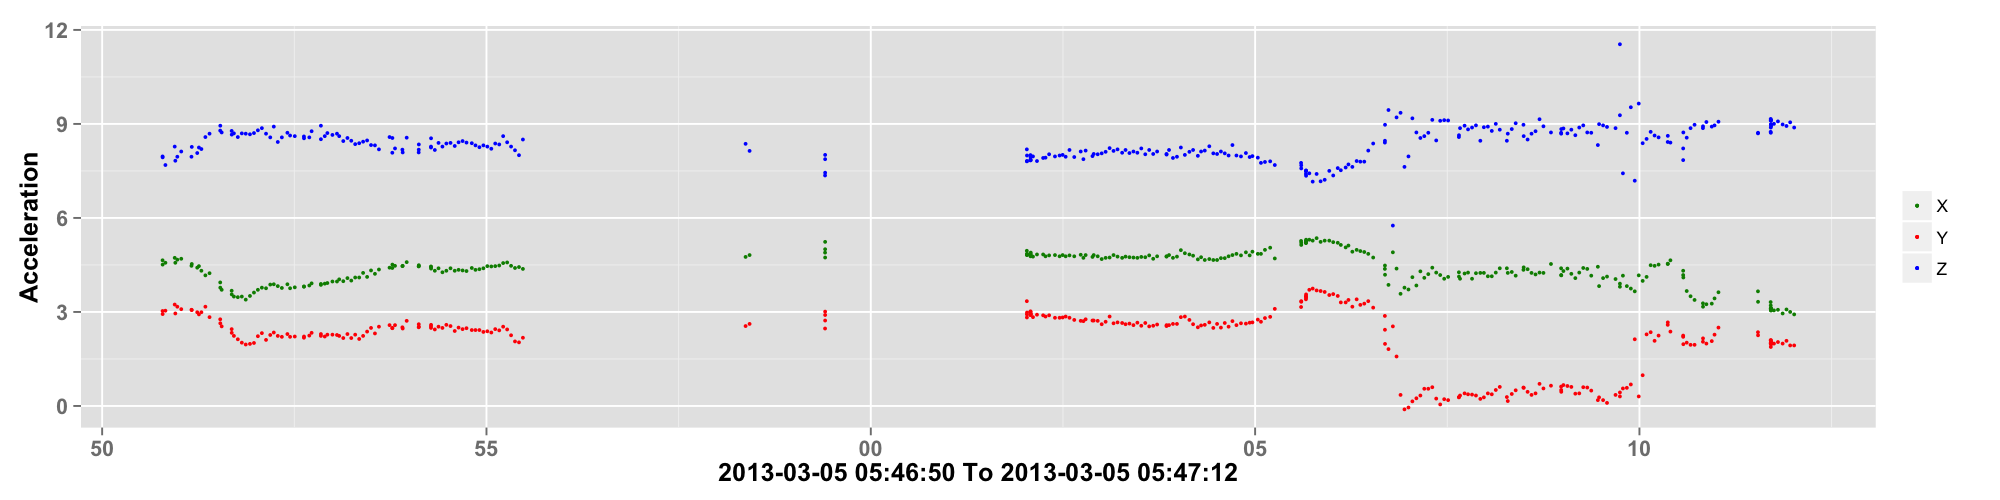
\includegraphics[width=1\textwidth]{photoshare/690194.png}}\\
		\subfloat[Sequence 838966]{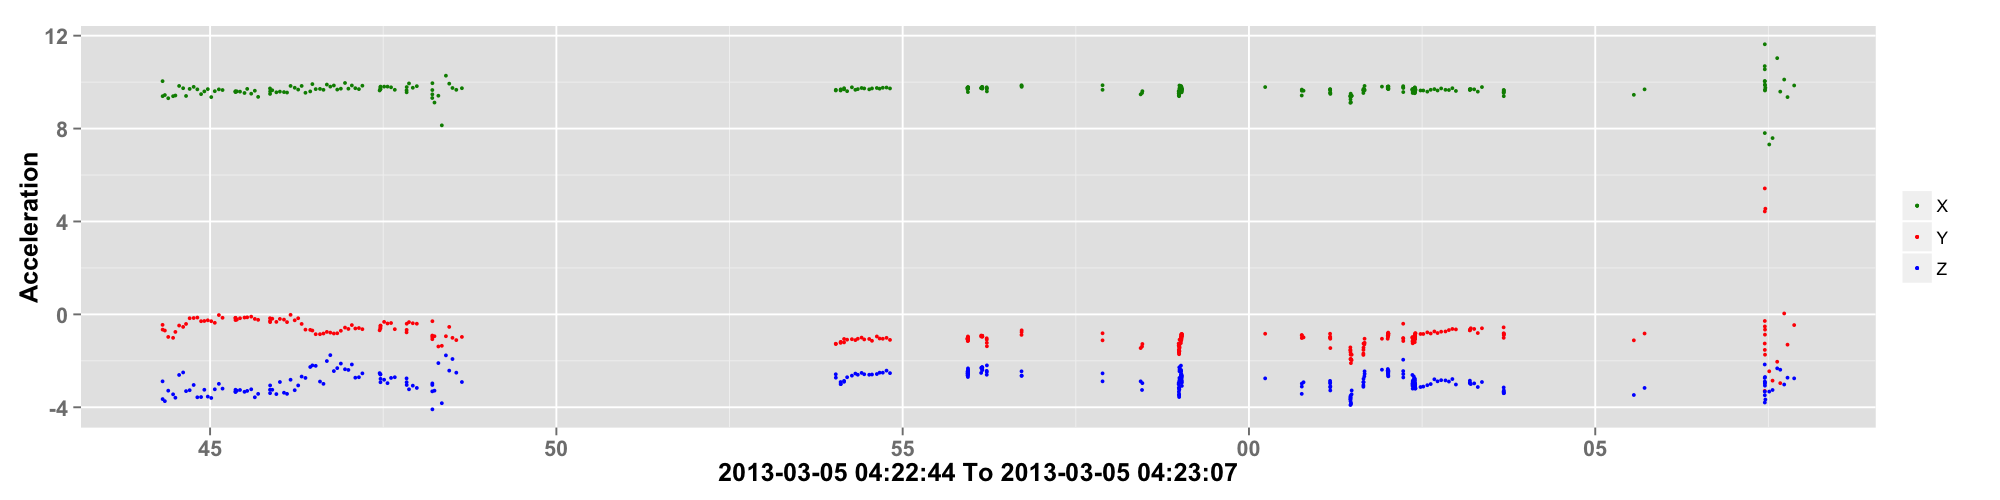
\includegraphics[width=1\textwidth]{photoshare/838966.png}}
		\caption{Test Sequence with Professed Device as 770}
	\end{figure}
	
	% section section_name (end)
	

	\section{Potential Approach} % (fold)
	\label{sec:potential_approach}
	\paragraph{}The data involve with time dimension, which is a very important feature. To solve this problem, an assumption should be made that users' activities have time-constraint re-occuring patterns, i.e. users are likely to have similar behavoir during roughly same time of day. For example, users would have similary X,Y and Z time series during today's 4:00 pm and yesterday's 4:00 pm. 
	\paragraph{} Based on this assumption, we design the following approaches:
	\begin{itemize}
		\item First, appropriate features from the raw data should be defined. Some simple but probably useful features include the range of X,Y,Z, the difference between X and Y, between X and Z, and between Y and Z, autocorrelation of X,Y and Z, and correlations between X,Y and Z, etc. In addition, We plan to do some literature research about what activities the data might reveal in order to extract features that represent users personal habbit such as how he/she runs. 
		\item Second, Supervised or Unsupervised?
			\begin{itemize}
			\item Treat it as a time-constrained classification problem, more specifically, a multi-classification problem, i.e. each device is a unique class. It seems that one-all should suffice this task. For a professed device Id, label 1 if true and 0 if its other device's Id. Since data are generated in different time intervals, training data might have different patterns during different time period. So given a test sequence $X_{test}$, we denote its time of day as $T_{test}$ (e.g. $T_{test}=19:00$). Then search all the training data and extract available training sequences (denote as $X_{train}$) that were fuzzily close to $T_{test}$. For the test sequence $X_{test}$, a professed device $D$ is known. We can label the training sequences from device $D$ as 1 and the training sequence from other device as 0. Based on the features we extract, train some classifiers with these training examples. Finally, apply the classifier to the test sequence to see wether it is 0 (test sequence is belong to other device) or 1 (test sequence is belong to device $D$).\\
			\item Learn a standardized ranking based probability metric indicating the similarity of a given test sequence and the associated training device. The heuristics behind this is if a test sequence comes from the claimed device, it should be most similar (defined by some similarity metrics like Euclidean distance, cosine similarity and so on) to this device instead of another. And the extracted features are only used to learn the weights of similarity features, which is different from a classification aaproach.
			\end{itemize}
	\end{itemize}
	Note: identifying what activity the test sequence represents such as running or walking or sleeping is also important. If the test sequence is from running but the running pattern from professed device is totally different with what test sequence reveals, then the professed device is probably a wrong device. 
	\paragraph{} We came up with these plots when we conducted exploratory data analysis, in each 2 by 2 plot, the top left graph comes from training data for a given device and the other 3 are sampled from test sequences that are claimed also from the given device.

	% \begin{figure}[ht]
	% 	\centering
	% 	\subfloat[Device 12]{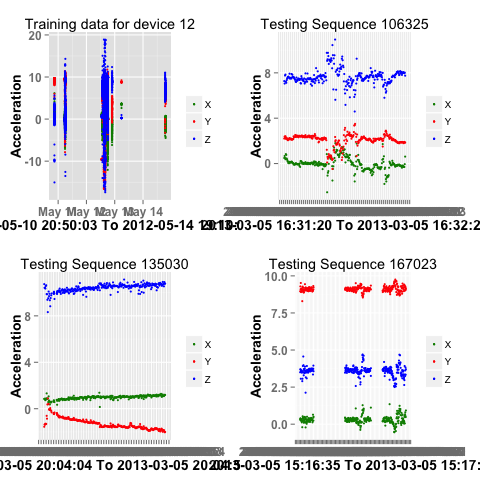
\includegraphics[width=1\textwidth]{photoshare/Device-12.png}}\\
	% 	%\subfloat[Device 12]{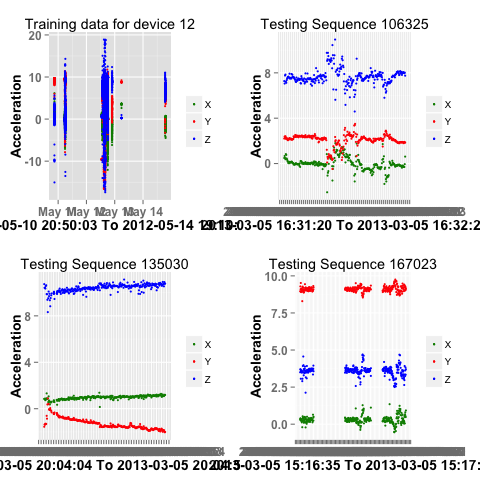
\includegraphics[width=1\textwidth]{photoshare/Device-12.png}}
	% 	\caption{Training data and test sequence labeled as Device 12}
	% \end{figure}



	\section{Timeline} % (fold)
	\label{sec:timeline}
	\begin{itemize}
		\item Research on literatures with acceleration data
		\item Extract important features 
		\item Initial result done (before the end of thanksgiving holiday)
		\item Discussion with instructors, improve results and write up
	\end{itemize}
	% section timeline (end)
	
	% section potential_approach (end)
	
\end{document}




